\documentclass[ucs,10pt]{beamer}

\usepackage[utf8x]{inputenc}    
\usepackage[english]{babel}    

% Template for talks using the Corporate Design of the Freie Universitaet
%   Berlin, created following the guidelines on www.fu-berlin.de/cd by
%   Tobias G. Pfeiffer, <tobias.pfeiffer@math.fu-berlin.de>
% This file can be redistributed and/or modified in any way you like.
%   If you feel you have done significant improvements to this template,
%   please consider providing your modified version to
%   https://www.mi.fu-berlin.de/w/Mi/BeamerTemplateCorporateDesign

\usepackage{amsmath,dsfont,listings}

%%% FU logo
% small version for upper right corner of normal pages
\pgfdeclareimage[height=0.9cm]{university-logo}{FULogo_RGB}
\logo{\pgfuseimage{university-logo}}
% large version for upper right corner of title page
\pgfdeclareimage[height=1.085cm]{big-university-logo}{FULogo_RGB}
\newcommand{\titleimage}[1]{\pgfdeclareimage[height=2.92cm]{title-image}{#1}}
\titlegraphic{\pgfuseimage{title-image}}
%%% end FU logo

% NOTE: 1cm = 0.393 in = 28.346 pt;    1 pt = 1/72 in = 0.0352 cm
\setbeamersize{text margin right=3.5mm, text margin left=7.5mm}  % text margin

% colors to be used
\definecolor{text-grey}{rgb}{0.45, 0.45, 0.45} % grey text on white background
\definecolor{bg-grey}{rgb}{0.66, 0.65, 0.60} % grey background (for white text)
\definecolor{fu-blue}{RGB}{0, 51, 102} % blue text
\definecolor{fu-green}{RGB}{153, 204, 0} % green text
\definecolor{fu-red}{RGB}{204, 0, 0} % red text (used by \alert)

% switch off the sidebars
% TODO: loading \useoutertheme{sidebar} (which is maybe wanted) also inserts
%   a sidebar on title page (unwanted), also indents the page title (unwanted?),
%   and duplicates the navigation symbols (unwanted)
\setbeamersize{sidebar width left=0cm, sidebar width right=0mm}
\setbeamertemplate{sidebar right}{}
\setbeamertemplate{sidebar left}{}
%    XOR
% \useoutertheme{sidebar}

% frame title
% is truncated before logo and splits on two lines
% if neccessary (or manually using \\)
\setbeamertemplate{frametitle}{%
    \vskip-30pt \color{text-grey}\large%
    \begin{minipage}[b][23pt]{80.5mm}%
    \flushleft\insertframetitle%
    \end{minipage}%
}

%%% title page
% TODO: get rid of the navigation symbols on the title page.
%   actually, \frame[plain] *should* remove them...
\setbeamertemplate{title page}{
% upper right: FU logo
\vskip2pt\hfill\pgfuseimage{big-university-logo} \\
\vskip6pt\hskip3pt
% title image of the presentation
\begin{minipage}{11.6cm}
\hspace{-1mm}\inserttitlegraphic
\end{minipage}

% set the title and the author
\vskip14pt
\parbox[top][1.35cm][c]{11cm}{\color{text-grey}\inserttitle \\ \small \insertsubtitle}
\vskip11pt
\parbox[top][1.35cm][c]{11cm}{\small \insertauthor \\ \insertinstitute \\[3mm] \insertdate}
}
%%% end title page

%%% colors
\usecolortheme{lily}
\setbeamercolor*{normal text}{fg=black,bg=white}
\setbeamercolor*{alerted text}{fg=fu-red}
\setbeamercolor*{example text}{fg=fu-green}
\setbeamercolor*{structure}{fg=fu-blue}

\setbeamercolor*{block title}{fg=white,bg=black!50}
\setbeamercolor*{block title alerted}{fg=white,bg=black!50}
\setbeamercolor*{block title example}{fg=white,bg=black!50}

\setbeamercolor*{block body}{bg=black!10}
\setbeamercolor*{block body alerted}{bg=black!10}
\setbeamercolor*{block body example}{bg=black!10}

\setbeamercolor{bibliography entry author}{fg=fu-blue}
% TODO: this doesn't work at all:
\setbeamercolor{bibliography entry journal}{fg=text-grey}

\setbeamercolor{item}{fg=fu-blue}
\setbeamercolor{navigation symbols}{fg=text-grey,bg=bg-grey}
%%% end colors

%%% headline
\setbeamertemplate{headline}{
\vskip4pt\hfill\insertlogo\hspace{3.5mm} % logo on the right

\vskip6pt\color{fu-blue}\rule{\textwidth}{0.4pt} % horizontal line
}
%%% end headline

%%% footline
\newcommand{\footlinetext}{\insertshortinstitute, \insertshorttitle, \insertshortdate}
\setbeamertemplate{footline}{
\vskip5pt\color{fu-blue}\rule{\textwidth}{0.4pt}\\ % horizontal line
\vskip2pt
\makebox[123mm]{\hspace{7.5mm}
\color{fu-blue}\footlinetext
\hfill \raisebox{-1pt}{\usebeamertemplate***{navigation symbols}}
\hfill \insertframenumber}
\vskip4pt
}
%%% end footline

%%% settings for listings package
\lstset{extendedchars=true, showstringspaces=false, basicstyle=\footnotesize\sffamily, tabsize=2, breaklines=true, breakindent=10pt, frame=l, columns=fullflexible}
\lstset{language=Java} % this sets the syntax highlighting
\lstset{mathescape=true} % this switches on $...$ substitution in code
% enables UTF-8 in source code:
\lstset{literate={ä}{{\"a}}1 {ö}{{\"o}}1 {ü}{{\"u}}1 {Ä}{{\"A}}1 {Ö}{{\"O}}1 {Ü}{{\"U}}1 {ß}{\ss}1}
%%% end listings  

%\usepackage{arev,t1enc} % looks nicer than the standard sans-serif font
% if you experience problems, comment out the line above and change
% the documentclass option "9pt" to "10pt"

% image to be shown on the title page (without file extension, should be pdf or png)
\titleimage{../graphics/quantumcomputingcover}

\title[Quantum-resistant signatures for IoT] % (optional, use only with long paper titles)
{Quantum-resistant digital signatures schemes for low-power IoT}

\author % (optional, use [] for lots of authors)
{H. Hattenbach}

\institute[FU Berlin] % (optional, but mostly needed)
{Freie Universität Berlin}

\date[] % (optional, should be abbreviation of conference name)
{Seminar Internet of Things, 2021}
% - Either use conference name or its abbreviation.
% - Not really informative to the audience, more for people (including
%   yourself) who are reading the slides online

\subject{Seminar Internet of Things}
% This is only inserted into the PDF information catalog. Can be left out.

% you can redefine the text shown in the footline. use a combination of
% \insertshortauthor, \insertshortinstitute, \insertshorttitle, \insertshortdate, ...
\renewcommand{\footlinetext}{\insertshortinstitute, \insertshorttitle, \insertshortdate}

% Delete this, if you do not want the table of contents to pop up at
% the beginning of each subsection:
\AtBeginSubsection[]
{
  \begin{frame}<beamer>{Outline}
    \tableofcontents[currentsection,currentsubsection]
  \end{frame}
}


\begin{document}

\begin{frame}[plain]
  \titlepage
\end{frame}

\begin{frame}{Outline}
  \tableofcontents[pausesections]
  % You might wish to add the option [pausesections]
\end{frame}

\section{Motivation}

\begin{frame}{Quantum Computing breaks ordinary Cryptography}
  % - A title should summarize the slide in an understandable fashion
  %   for anyone how does not follow everything on the slide itself.
  \begin{itemize}
  \item
    sufficiently sized Quantum Computers (explained later) on the horizon
  \item
    They can break most of the cryptography in current use
    \begin{itemize}
      \item RSA
      \item ECDSA / ECDH
      \item $\rightarrow$ Signal, WhatsApp, PGP, SSH, TLS/HTTPS, \dots
    \end{itemize}
  \item 
    not everything equally effected
    \begin{itemize}
      \item schemes in standardization to replace current cryptography
      \item some are rather computationally intense
      \item that is why i have a deeper look on which are feasable for IoT
    \end{itemize}
  \end{itemize}
\end{frame}

\subsection{Quantum Computing}

\begin{frame}{Shors algorithm poses threat against asymmetric cryptography}
  % - A title should summarize the slide in an understandable fashion
  %   for anyone how does not follow everything on the slide itself.
  \begin{itemize}
  \item
    Quantum Computers operate on Qubits instead of normal Bits
  \item
    Qubits are Quantum-Mechanical
    \begin{itemize}
      \item using spin of an electrons
      \item Entanglement and Superposition
    \end{itemize}
  \item
    Algorithms can leverage those mechanics
    \begin{itemize}
      \item up to exponential speed up in some cases
      \item Shors algorithm completely breaks common asymmetric cryptography
      \begin{itemize}
        \item can derive private key from public key
        \item for everything based on Number-Theory (like RSA, ECDSA, ..)
      \end{itemize}
      \item  Grovers algorithm poses threat against symmetric crypto and hash-functions
      \begin{itemize}
        \item only quadratic speed-up
        \item doubling length restores security (e.g. AES128 $\mapsto$ AES256)
      \end{itemize}
    \end{itemize}
  \end{itemize}
\end{frame}


\begin{frame}{Shors algorithm poses threat against asymmetric cryptography}
  % - A title should summarize the slide in an understandable fashion
  %   for anyone how does not follow everything on the slide itself.
  \begin{itemize}
  \item
    Quantum Computers operate on Qubits instead of normal Bits
  \begin{figure}[htbp]
    \centering
    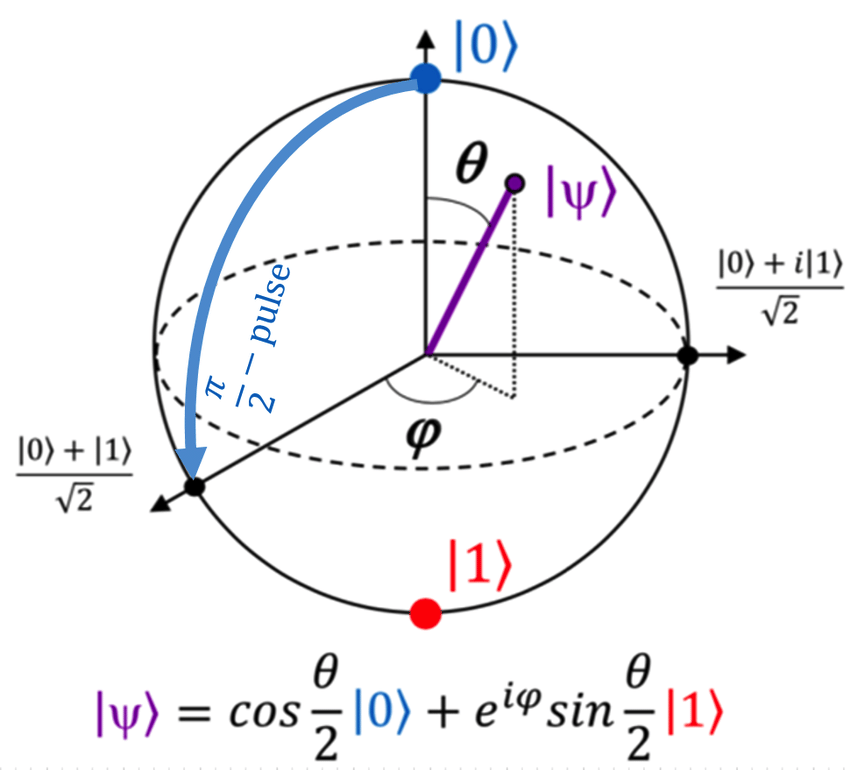
\includegraphics[width=.2\textwidth]{../graphics/The-Bloch-sphere-provides-a-useful-means-of-visualizing-the-state-of-a-single-qubit-and.png}
    \caption{Model of a Qubit \cite{img:bloch}}
    \label{qubit}
  \end{figure}
  \item
    Algorithms can leverage those mechanics
    \begin{itemize}
      \item up to exponential speed up in some cases
      \item Shors algorithm completely breaks common asymmetric cryptography
      \begin{itemize}
        \item can derive private key from public key
        \item for everything based on Number-Theory (like RSA, ECDSA, ..)
      \end{itemize}
      \item  Grovers algorithm poses threat against symmetric crypto and hash-functions
      \begin{itemize}
        \item only quadratic speed-up
        \item doubling length restores security (e.g. AES128 $\mapsto$ AES256)
      \end{itemize}
    \end{itemize}
  \end{itemize}
\end{frame}

\begin{frame}
  \frametitle{Shors and Grovers algorithms}
    \begin{figure}[htbp]
      \centering
      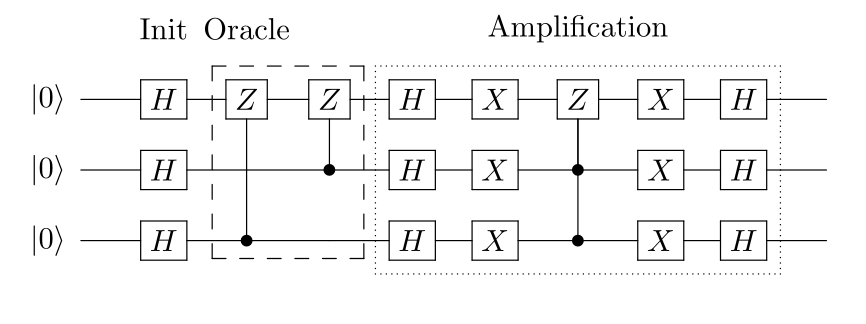
\includegraphics[width=.7\textwidth]{../graphics/grover_circuit_3qubits.png}
      \caption{Grovers Algorithm \cite{img:grover}}
      \label{grover}
    \end{figure}
  
    \begin{figure}[htbp]
      \centering
      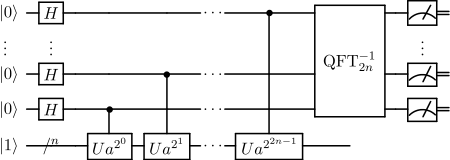
\includegraphics[width=.5\textwidth]{../graphics/Shor's_algorithm.png}
      \caption{Shors Algorithm\cite{img:shor}}
      \label{shor}
    \end{figure}

\end{frame}

\subsection{Internet of Things}

\begin{frame}{Many ressource constrained devices}
  % - A title should summarize the slide in an understandable fashion
  %   for anyone how does not follow everything on the slide itself.
  \begin{itemize}
  \item
    Internet of Things 
  \item
    Smart-devices that are actually pretty dumb
    \begin{itemize}
      \item little memory (kilobytes to megabytes)
      \item low computing power (slow clock, small cache, etc.)
      \item limited energy ressources (battery or solar operated)
    \end{itemize}
  \item
    NIST classified into 3 classes:
  \end{itemize}
  \begin{table}
    \label{IoT-classes}
    \centering
    \caption{IETF IoT Classes}
    \begin{tabular}{|l | c c|}
        \hline
        Class & RAM & Flash \\
        \hline
        C0 & $<<$ 10 KiB & $<<$ 100 KiB\\
        C1 & ~ 10 KiB & ~ 100 KiB\\
        C2 & ~ 50 KiB & ~ 250 KiB\\
        \hline
    \end{tabular} 
\end{table}
\end{frame}

\section{Quantum Resistant Signature Schemes}

\subsection{Performance Metrics}
\begin{frame}{What makes a signature scheme better than any other?}

  \begin{itemize}
  \item length of:
  \begin{itemize}
    \item signature
    \item public key
    \item private key
  \end{itemize}
    \item time and space needed to:
    \begin{itemize}
      \item generate keys (GEN)
      \item sign a message (SIGN)
      \item verify a message (VER)
    \end{itemize}
  \item security against quantum computers and traditional attackers
  \begin{table}
    \label{QR-classes}
    \centering
    \caption{QR Security classes and their traditional counterparts as classified by the NIST}
    \begin{tabular}{|l | c|}
        \hline
        Class & security comparable to \\
        \hline
        1 & AES-128 \\
        2 & SHA256 \\
        3 & AES-192 \\
        4 & SHA384 \\
        5 & AES-256 \\
        \hline
    \end{tabular} 
\end{table}
\end{itemize}
\end{frame}

\subsection{different types}
\begin{frame}{Multiple types of underlying mathematica problems}

  \begin{itemize}
    \item Super-singular isogeny based
    \begin{itemize}
      \item SIKE
      \item not well studied
    \end{itemize}
    \item Multivariate polynomial based
    \begin{itemize}
      \item Rainbow
      \item not well studied
      \item involves guessing work $\rightarrow$ not suited for low power devices
    \end{itemize}
    \item Code based
    \begin{itemize}
      \item McEliece
      \item no finalist
    \end{itemize}
    \item Hash based
    \begin{itemize}
      \item SPHINCS+ 
      \item big signatures (see next slide)
      \item very well studied
    \end{itemize}
    \item Lattice based
    \begin{itemize}
      \item FALCON, Dilithium
      \item most promising
      \item most NIST finalists
      \item most efficient
      \item not as proofed as HBS
    \end{itemize}
  \end{itemize}
  

\end{frame}


\section{Structure}
\subsection{Skeleton}

\begin{frame}{Skeleton}
  \begin{itemize}
      \item Introduction
    
      \item Internet of Things
      
      \item Quantum Resistant Security
          \begin{itemize}
            \item Quantum Computing
            \item QR Algorithms
            \begin{itemize}
              \item Performance Metrics
              \item Encryption
              \item Signatures
            \end{itemize}
          \end{itemize}
      
      \item QR Signatures in IoT 
      \begin{itemize}
        \item Performance Metrics in IoT
        \item Failed Signatures
        \begin{itemize}
          \item WalnutDSA
          \item qTESLA
        \end{itemize}
        \item FALCON
      \end{itemize}
      
      
      \item {Conclusion}
  \end{itemize}
  
\end{frame}

\subsection{Width-Covorage}
\begin{frame}{Creating an Overview}
  \begin{itemize}
    \item Skimming multiple Quantum Resistant (QR) algorithms \cite{QR_algs,PQClean-GH} that focus on IoT \cite{QR_comparison,Energy_comp,QR_Iot_Lattice,QR_IoT,QR_IoT_Energy} 
    \item Deeper reserach about signature Schemes \cite{QR_sigs}
    \item and having a slightly more detailed look at two failed sschemes \cite{WalnutDSA,WalnutDSA_broken,qtesla,qtesla_masked}
    
  \end{itemize}
\end{frame}

\subsection{Depth-Covorage}
\begin{frame}{Diving Deeper}
  \begin{itemize}
    \item  having a deeper look at a NIST QR finalist with the most compact implementation:

    FALCON \cite{falcon_and_dilithium,falcon_micro_impl,bearz}
   
    \item  maybe having an outlook in the end on a Hardware-Accelerated QR chip \cite{IoT_ASIC} 
  \end{itemize}

\end{frame}

\subsection{Ressources}
\begin{frame}[allowframebreaks]{Ressources}
  \bibliographystyle{plain}
  %\bibliography{img}
  \bibliography{img.bib, ../lit.bib}
\end{frame}

\subsection{Schedule}
\begin{frame}{Planned Schedule}
\begin{itemize}
  \item 7.5. : skim breadth coverage literature
  \item 15.5.: write until signatures (at least bullet point comments)
  \item 30.5.: finish breadth (at least bullet point comments)
  \item $\alpha$: skim and bullet point Depth
  \item 30.6.: finish
\end{itemize}
\end{frame}

\end{document}

